\documentclass[12pt,aspectratio=169]{beamer}

\usetheme[progressbar=frametitle, numbering=fraction]{metropolis}
\usepackage{appendixnumberbeamer}
\usepackage{minted}
\usepackage{booktabs}
%\usepackage[scale=2]{ccicons}
\usepackage{amsmath}
\usepackage{pgfplots}
\usepgfplotslibrary{dateplot}
\usepackage{multicol}
\usepackage{xspace}

%\usepackage[fontset=ubuntu]{ctex}


% Math Fonts
\usefonttheme{professionalfonts}
%\usepackage{mathspec}
%\setsansfont[BoldFont={Fira Sans},Numbers={OldStyle}]{Fira Sans Light}
%\setmathsfont(Digits)[Numbers={Lining, Proportional}]{Fira Sans Light}

% Change Color of the theme
\usepackage{xcolor}
\definecolor{DarkGrey}{HTML}{353535}
\definecolor{ECNURed}{RGB}{164,31,53}
\definecolor{ECNUBrown}{RGB}{134,117,77}
\setbeamercolor{normal text}{ fg= DarkGrey  }
\setbeamercolor{alerted text}{ fg= ECNURed  }
\setbeamercolor{example text}{ fg= ECNUBrown  }

% Bolder Fonts for presenting in a large room 
%\setsansfont[BoldFont={Fira Sans SemiBold}]{Fira Sans Book}
\setbeamertemplate{footline}[transparent]
\setbeamertemplate{footline}[frame number]
\setbeamerfont{footnote}{size=\scriptsize}
%---------------------commands

%\emph{emphasize}
%\alert{accent}
%\textbf{bold}

\newcommand{\themename}{\textbf{\textsc{metropolis}}\xspace}
\newcommand{\cg}[1]{
\colorbox{gray!30}{#1}
}
\newcommand{\f}[2]{
\metroset{titleformat frame=regular}
\begin{frame}{#1}
#2
\end{frame}
}

\newcommand{\fnum}[2]{
\f{#1}{
\addtocounter{framenumber}{-1}
#2
}
}

\newcommand{\footurl}[1]{
{
\footnote{\url{#1}}
}
}

\newcommand{\js}{JavaScript
}

\newcommand{\node}{Node.js
}

\newcommand{\figsize}{6cm}

\newcommand{\fig}[2]{
\begin{center}
    \fbox{
    \includegraphics[height=#1]{#2}
    }   
\end{center}
}

\newcommand{\figu}[2]{
\begin{figure}[H]
\fbox{
\includegraphics[height=#1]{#2}
}
\end{figure}
}

\newcommand{\inputcode}[3]{
\metroset{block=fill}
\begin{block}{#1}
    \inputminted{#2}{#3}
\end{block}
}

\newcommand{\icode}[3]{
\metroset{block=fill}
\begin{block}{#1}
    \begin{minted}{#2}
    #3
    \end{minted}
\end{block}
}

\newcommand{\fq}{
{
\setbeamercolor{palette primary}{fg=black, bg=white}
\begin{frame}[standout]
  Questions ?
\end{frame}
}
}

%---------------------------

\title{WEB101}
\subtitle{Bases du développement web}
\date{2022}
\author{Nans WEBERT (n4n5)}
\institute{Télécom Paris}
\titlegraphic{
    \hfill
    
\includegraphics[height=1.5cm]{data/imgs/rezel.png}
}

\begin{document}

\maketitle

\f{Sommaire}{
  \setbeamertemplate{section in toc}[sections numbered]
  \tableofcontents[hideallsubsections]
}

\f{Sommaire}{
Qui suis-je ?
\begin{itemize}
    \item Télécom Paris - Groupe 6 (DUT R\&T)
    \item 1 an d'alternance - développeur Full Stack \js
\end{itemize}
Pourquoi ce "cours" ?
\begin{itemize}
    \item votre PACT ?
    \item \js > all
    \item votre curiosité
\end{itemize}
}

\section{Introduction au web}

\f{Rappel HTTP - Vue protocole}{
\begin{columns}
\begin{column}{0.5\textwidth}
    \figu{5cm}{data/imgs/osi_http.png}
\end{column}
\begin{column}{0.5\textwidth}
    HTTP = couche "Application"\\
    Sur la couche "Transport" :
    \begin{itemize}
        \item \cg{TCP}
        \item \cg{UDP}
    \end{itemize}
\end{column}
\end{columns}
\footurl{https://fr.wikipedia.org/wiki/QUIC}
}


\f{Rappel HTTP - Communication}{
\begin{center}
\fig{5cm}{data/imgs/http-communication.png}\cite{http-com}\footnote{Mais aussi avec plusieurs serveurs !}
\end{center}
}

\f{Rappel HTTP - Protocole}{
Plusieurs versions :
\begin{itemize}
    \item \cg{HTTP/1.1}
    \item \cg{HTTP/2}
    \item \cg{HTTP/3} (over QUIC)
\end{itemize}
Qu'est-ce que HTTPS ?\\
$$HTTPS = HTTP + TLS$$\\
(TLS au dessus de HTTP)
}



\f{Rappel HTTP - Requetes}{
Types de requêtes :
\begin{itemize}
    \item \cg{GET}
    \item \cg{POST}
    \item \cg{PUT}
    \item bien d'autres : \cg{DELETE}, \cg{OPTIONS}, \cg{HEAD} ... \footurl{https://developer.mozilla.org/fr/docs/Web/HTTP/Methods}
\end{itemize}
}

\f{Rappel HTTP - Requetes}{
Types de réponses :
\begin{itemize}
    \item \cg{200 OK}
    \item \cg{404 Not Found}
    \item \cg{500 Internal Server Error}
    \item \cg{301 Moved Permanently}
    \item bien d'autres : \cg{204 ...}, \cg{403 ..}, \cg{418 ...} etc \footurl{https://developer.mozilla.org/fr/docs/Web/HTTP/Status}
\end{itemize}
}

\f{Rappel HTTP - Headers}{
\metroset{block=fill}
\centering
\begin{block}{Analyse d'une requête web}
curl --verbose http://info.cern.ch/hypertext/WWW/TheProject.html
\end{block}
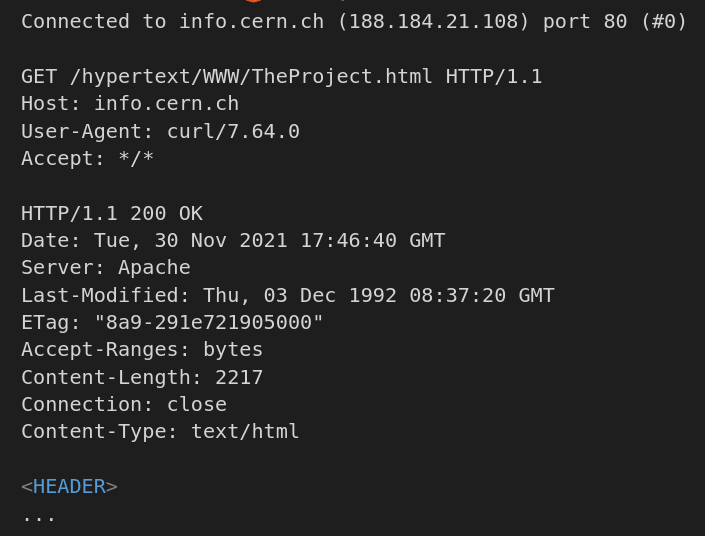
\includegraphics[width=7cm]{./data/imgs/curl_request.png}
}

\fnum{Rappel HTTP - Headers}{
\begin{center}
    Les headers
    \fig{5.5cm}{data/imgs/curl_request.png}
\end{center}
}

\fnum{Rappel HTML - CSS}{
\begin{columns}
\begin{column}{0.5\textwidth}
{\scriptsize
    \inputcode{HTML}{html}{data/code/html.tex}
}
\end{column}
\begin{column}{0.5\textwidth}
{\scriptsize
    \inputcode{CSS}{css}{data/code/css.tex}
}
\end{column}
\end{columns}
}

\f{Comment faire un site ?}{
Comment faire un site ?
\begin{itemize}
    \item Avec un serveur qui renvoie les pages
\end{itemize}
}

\f{Comment faire un site ?}{
Comment faire un site dynamique ?
\begin{itemize}
    \item Avec un serveur qui exécute un programme qui renvoi une page, on utilise la \cg{CGI}\footurl{https://fr.wikipedia.org/wiki/Common_Gateway_Interface}
\end{itemize}
}

\fnum{Comment faire un site ?}{
\begin{center}
En C
\small
\inputcode{c CGI}{c}{data/code/server/c-cgi.tex}
\end{center}
}

\fnum{Comment faire un site ?}{
\begin{center}
En PHP
\small
\inputcode{PHP webserver}{php}{data/code/server/php.tex}
\end{center}
}

\fnum{Comment faire un site ?}{
\begin{center}
En Python : \cite{python-webserver}
\tiny
\inputcode{Python webserver}{python}{data/code/server/python.tex}
\end{center}
}

\fnum{Comment faire un site ?}{
\begin{center}
En \node :
\inputcode{\node web server}{js}{data/code/server/nodejs.tex}
\end{center}
}

\f{Comment faire un site ?}{
On fait moins travailler le serveur:
\begin{itemize}
    \item Faire le rendu côté client\footnote{\cg{CSR} : Client-Side Rendering} !
\end{itemize}
}

\f{Comment faire un site ?}{
Mais le rendu client peut être lent !
\begin{itemize}
    \item On pré-rend les pages webs : \cg{SSG}\footnote{Static Site Generation, on rend seule fois}, \cg{SSR} \footnote{Server Side Rendering (on a ensuite des concepts tel que l'\cg{hydratation})}
\end{itemize}
{
\scriptsize
Plus d'informations :
\begin{itemize}
    \item \url{https://developers.google.com/web/updates/2019/02/rendering-on-the-web}
    \item à la fin du diapo
\end{itemize}
}
}

\fq

\section{\js}

\f{\js}{
\js c'est :
\begin{itemize}
    \item pas JAVA
    \item créé en 1995
    \item "The World's Most Misunderstood Programming Language" \footurl{https://www.crockford.com/javascript/javascript.html}
    \item le V8 \js Engine \footurl{https://v8.dev}
    \item plus de problème de points-virgules !
\end{itemize}
}

\fnum{\js}{
Où est-il ?
\begin{itemize}
    \item dans le navigateur
    \item sur un serveur - NodeJS et Deno
    \item sur un logiciel Desktop - Electron
    \item sur un smartphone - ReactNative...
\end{itemize}
}

\f{Navigateur}{
Tour du propriétaire d'un navigateur web
\newline
\newline
Afficher l'inspecteur web :
\begin{itemize}
    \item \cg{CTRL} + \cg{MAJ} + \cg{I}
    \item Clique droit > \cg{Inspecter}
\end{itemize}
}

\fnum{Navigateur}{
Tour du propriétaire d'un navigateur web : l'\cg{inspecteur}
\fig{\figsize}{data/imgs/inspector.png}
}

\fnum{Navigateur}{
Tour du propriétaire d'un navigateur web : l'onglet \cg{console}
\fig{\figsize}{data/imgs/console.png}
}

\fnum{Navigateur}{
Tour du propriétaire d'un navigateur web : l'onglet \cg{network}
\fig{\figsize}{data/imgs/network.png}
}

\fnum{Navigateur}{
Tour du propriétaire d'un navigateur web : l'onglet \cg{sources}
\fig{\figsize}{data/imgs/sources.png}
}

\fnum{Navigateur}{
Tour du propriétaire d'un navigateur web : l'onglet \cg{application}
\fig{\figsize}{data/imgs/application.png}
}

\f{\js}{
Comment faire du \js dans un navigateur ?
\begin{itemize}
    \item depuis la console
    \item dans le HTML
    \item dans un fichier \cg{*.js}
    \item via une extension
    \item via un favoris \footurl{https://chriszarate.github.io/bookmarkleter/}
\end{itemize}
}

\f{\js - dans la console}{
\fig{7cm}{data/imgs/console_usage.png}
}

\f{\js - dans la console}{
\fig{2cm}{data/imgs/console_usage_2.png}
}

\f{\js - dans le HTML}{
\inputcode{\js dans le HTML}{html}{data/code/js-in-html.tex}
}

\f{\js - dans un fichier}{
\inputcode{\js dans un fichier externe}{html}{data/code/js-in-file.tex}
}

\f{\js - dans un fichier}{
\inputcode{\js dans un fichier externe}{html}{data/code/js-in-file-2.tex}
}


\f{Framework vs librairie}{
\begin{center}
Utiliser un framework ?
\end{center}
}

\fnum{Framework vs librairie}{
\begin{center}
Utiliser un framework ?
\fig{4cm}{data/imgs/framework.png}
Framework vs librairie\footurl{https://kobaltsolutions.com/framework-vs-library/}
\end{center}
}

\f{\js - Référence}{
\begin{center}
\large
\url{https://developer.mozilla.org/}
\end{center}
}

\f{\js - variables}{
\inputcode{Les différentes variables}{js}{data/code/js/js-var.tex}
\footnote{\cg{let} et \cg{var} ont des scopes différents}
}

\f{\js - constante}{
\inputcode{Définition d'une constante}{js}{data/code/js/js-const.tex}
}


\f{\js - tableau (array)}{
\inputcode{\js : tableau}{js}{data/code/js/js-array.tex}
}

\f{\js - objet (object) }{
\inputcode{\js : objet}{js}{data/code/js/js-object.tex}
}

\f{\js - constante}{
\inputcode{Définition d'une constante}{js}{data/code/js/js-const-2.tex}
}

\f{\js - objet (object) }{
\inputcode{\js objet}{js}{data/code/js/js-loop.tex}
}

\f{\js - objet (object) }{
\inputcode{\js : objet}{js}{data/code/js/js-loop-2.tex}
}

\f{\js - Destructuring et spread }{
\inputcode{\js : Destructuring}{js}{data/code/js/js-destructuring.tex}
}

\f{\js - Destructuring et spread }{
\inputcode{\js : Destructuring}{js}{data/code/js/js-destructuring-2.tex}
}

\f{\js - Destructuring et spread }{
\inputcode{\js : Spread}{js}{data/code/js/js-spread.tex}
}

\f{\js - Destructuring et spread }{
\inputcode{\js : Spread}{js}{data/code/js/js-spread-2.tex}
}

\f{\js - fonction }{
\inputcode{Fonction simple}{js}{data/code/js/js-func.tex}
}

\f{\js - fonction}{
\inputcode{Fonction dans une variable}{js}{data/code/js/js-func-2.tex}
}

\f{\js - fonction }{
\inputcode{Fonction fléchée (arrow function)}{js}{data/code/js/js-func-3.tex}
}

\f{\js - fonction }{
\small
\inputcode{Fonction fléchée (arrow function) minimale}{js}{data/code/js/js-func-4.tex}
}

\f{\js - Fonctions usuelles }{
\small
\inputcode{Fonction utiles}{js}{data/code/js/js-func-use.tex}
}

\f{\js - Méthodes sur les tableaux }{
\inputcode{Méthodes de manipulation d'un tableau}{js}{data/code/js/js-array-func.tex}
}

\fnum{\js - Méthodes sur les tableaux }{
\inputcode{Méthodes de manipulation d'un tableau}{js}{data/code/js/js-array-func-2.tex}
}

\fnum{\js - Méthodes sur les tableaux }{
\inputcode{Méthodes de manipulation d'un tableau}{js}{data/code/js/js-array-func-3.tex}
}

\fnum{\js - Méthodes sur les tableaux }{
\inputcode{Méthodes de manipulation d'un tableau}{js}{data/code/js/js-array-func-4.tex}
}

\f{\js}{
\begin{center}
    JavaScript, un langage monothread
    \inputcode{[Tuto] - comment faire crasher un onglet}{js}{data/code/monothread.tex}
\end{center}
}

\f{\js - Promises}{
\inputcode{Promesses (Promises)}{js}{data/code/js/js-promise.tex}
}
\fnum{\js - Promises}{
\inputcode{Promesses (Promises)}{js}{data/code/js/js-promise-2.tex}
}
\fnum{\js - Promises}{
\small
\inputcode{Promesses (Promises)}{js}{data/code/js/js-promise-3.tex}
}
\fnum{\js - Promises}{
\small
\inputcode{Promesses (Promises)}{js}{data/code/js/js-promise-4.tex}
}
\fnum{\js - Promises}{
\footnotesize
\inputcode{Promesses (Promises)}{js}{data/code/js/js-promise-5.tex}
}
\fnum{\js - Promises}{
\footnotesize
\inputcode{Promesses (Promises)}{js}{data/code/js/js-promise-6.tex}
}

\section{\js dans le navigateur}

\f{\js - DOM}{
Document Object Model (DOM)\cite{js-dom}
\fig{5cm}{data/imgs/dom.png}
}

\f{\js - utilisation du DOM}{
\inputcode{Naviguer dans le DOM}{js}{data/code/js/js-dom.tex}
}

\fnum{\js - utilisation du DOM}{
\small
\inputcode{Naviguer dans le DOM}{js}{data/code/js/js-dom-2.tex}
}

\fnum{\js - Web API}{
Comment ça marche : Web API \footurl{https://developer.mozilla.org/en-US/docs/Web/API}
\begin{itemize}
    \item \cg{fetch}
    \item \cg{window}
    \begin{itemize}
        \item  \cg{localStorage}
        \item \cg{sessionStorage}
    \end{itemize}
    \item \cg{document}
    \item \cg{canvas API}
    \item et d'autres : \cg{Intersection Observer API}, \cg{Sensor API}...
\end{itemize}
}

\fnum{\js - Events}{
\small
\inputcode{Events}{js}{data/code/js/js-events-1.tex}
Cela pose un problème !
}

\fnum{\js - Events}{
\small
\inputcode{Events}{js}{data/code/js/js-events-2.tex}
On peut mettre plusieurs events !
}

\f{\js - Frameworks}{
Frameworks
\begin{itemize}
    \item ReactJS
    \item VueJS
    \item SvelteJS
    \item AngularJS
\end{itemize}
}

\fnum{\js - Frameworks}{
ReactJS \footnote{Un nouveau langage : le \cg{JSX} (JavaScript Syntax eXtension) }
\tiny
\inputcode{ReactJS - Hello World}{tex}{data/code/js-example/react.tex}
}

\fnum{\js - Frameworks}{
VueJS
\tiny
\inputcode{VueJS - Hello World}{tex}{data/code/js-example/vuejs.tex}
}

\fnum{\js - Frameworks}{
Svelte\footnote{Besoin d'être "compilé"}
\inputcode{Events}{tex}{data/code/js-example/svelte.tex}
}

\fnum{\js - Frameworks}{
Angular :(
\begin{center}
    \url{https://stackblitz.com/fork/angular-ivy}
\end{center}
}


\fq

\section{\node}

\f{\node}{
\node :
\begin{itemize}
    \item créé en 2009 par Ryan Dahl (créateur de Deno, en 2018)
    \item concept : utiliser le moteur V8 à l'extérieur du navigateur
\end{itemize}
}

\f{Visual Studio Code}{
\begin{center}
Une IDE très performant, fait lui-même en \js\newline

\includegraphics[width=1cm]{data/imgs/vscode/vscode_logo.png}\\
\url{https://code.visualstudio.com/}
\end{center}
}

\f{Visual Studio Code}{
\fig{\figsize}{data/imgs/vscode/vscode.png}
}

\f{Visual Studio Code}{
\begin{center}
    Débugger sur VSCode
\end{center}
}

\fnum{Visual Studio Code}{
\centering
\cg{Terminal} > \cg{New Terminal}
\fig{3.5cm}{data/imgs/vscode/terminal.png}
}

\fnum{Visual Studio Code}{
\centering
\cg{+} > \cg{\js Debugger Terminal}
\fig{3.5cm}{data/imgs/vscode/terminal-debug.png}
}

\f{Visual Studio Code}{
\centering
\fig{5.8cm}{data/imgs/vscode/debugging.png}
}

\f{Visual Studio Code}{
\begin{center}
    Débugger sur VSCode, autre méthode :
    \begin{itemize}
        \item \cg{Run and Debug (Ctrl + Shift + D)}
        \item \cg{Create a launch.json file} (il sera créer dans \cg{.vscode/launch.json})
        \item Modifier le \cg{launch.json} par exemple pour ajouter d'autres attributs (facultatif)
        \item \cg{F5} pour débugger
    \end{itemize}
\end{center}
}

\fnum{Visual Studio Code}{
\tiny
\inputcode{launch.json}{json}{data/code/launch.tex}
}


\f{\js - NPM}{
Commencer un projet :
\begin{itemize}
    \item npm init
    \item licence
    \item installer des packages
    \item faire des scripts
\end{itemize}
\inputcode{npm init}{sh}{data/code/npm/npm-init.tex}
}

\f{\js - NPM}{
Créer un projet :
\begin{itemize}
    \item npm init\footnote{installer \cg{npm} si non-présent}
\end{itemize}

\inputcode{npm init}{sh}{data/code/npm/npm-init.tex}
}

\f{\js - NPM}{
\small
\inputcode{npm init créer un fichier \cg{package.json}}{json}{data/code/npm/init.tex}
}

\f{\js - NPM}{
Commencer un projet :
\begin{itemize}
    \item npm init \checkmark
    \item licence
\end{itemize}
\begin{center}
La licence\footnote{Un lien utile : \url{https://choosealicense.com/licenses/}} est à mettre dans le \cg{package.json} à l'attribut \cg{license}\footurl{https://spdx.org/licenses/}
\end{center}
}

\fnum{\js - NPM}{
\begin{itemize}
    \item npm init \checkmark
    \item licence \checkmark
    \item installer des packages
\end{itemize}
\inputcode{Package}{js}{data/code/npm/commands.tex}
}

\fnum{\js - NPM}{
Après la commande \cg{npm add axios}
\scriptsize
\inputcode{Package - dependencies}{js}{data/code/npm/init-2.tex}
}

\fnum{\js - NPM}{
Après la commande \cg{npm add --save-dev mocha}
\scriptsize
\inputcode{Package - dev dependencies}{js}{data/code/npm/init-3.tex}
}

\fnum{\js - NPM}{
\begin{itemize}
    \item npm init \checkmark
    \item licence \checkmark
    \item installer des packages \checkmark
    \item faire des scripts
\end{itemize}
\inputcode{npm run}{sh}{data/code/npm/npm-run.tex}
}

\fnum{\js - NPM}{
\scriptsize
\inputcode{npm run}{sh}{data/code/npm/init-4.tex}
}

\f{\js - \node}{
\begin{center}
    Développement en \node
\end{center}
}

\f{\js - \node}{
\begin{center}
    Toujours monothread ! -> Notion d'Event Loop \cite{event-loop}
    \fig{4.5cm}{data/imgs/event-loop.png}
    Longue opérations -> en \cg{async}
\end{center}
}

\f{\js - \node}{
Les modules :
\begin{itemize}
    \item Core Modules (\cg{http}, \cg{path}, \cg{fs})
    \item NPM Modules \footurl{https://www.npmjs.com/}
\end{itemize}
\inputcode{Module quelconque}{js}{data/code/nodejs/module.tex}
}

\f{\js - \node}{
Les modules, deux normes :
\begin{itemize}
    \item CommonJS
    \inputcode{Import CommonJS}{js}{data/code/nodejs/module.tex}
    \item ES6 (standard) \footnote{il faut l'attribut \cg{"type": "module"} dans le \cg{package.json}}
    \inputcode{Import ES6}{js}{data/code/nodejs/module-2.tex}
\end{itemize}
}

\f{\js - \node}{
Que se passe-t-il quand on \cg{require} un fichier ?
\begin{columns}
\begin{column}{0.5\textwidth}
    {\tiny
    \inputcode{myModule.js}{js}{data/code/nodejs/require-1bis.tex}
    }
\end{column}
\begin{column}{0.5\textwidth}  %%<--- here
    {\tiny
    \inputcode{index.js}{js}{data/code/nodejs/require-1.tex}
    }
\end{column}
\end{columns}
}


\fnum{\js - \node}{
Que se passe-t-il quand on \cg{require} un fichier ?
\begin{columns}
\begin{column}{0.5\textwidth}
    {\tiny
    \inputcode{myModule.js}{js}{data/code/nodejs/require-2bis.tex}
    }
\end{column}
\begin{column}{0.5\textwidth}  %%<--- here
    {\tiny
    \inputcode{index.js}{js}{data/code/nodejs/require-2.tex}
    }
\end{column}
\end{columns}
}

\fnum{\js - \node}{
Que se passe-t-il quand on \cg{require} un fichier ?
\begin{columns}
\begin{column}{0.5\textwidth}
    {\tiny
    \inputcode{myModule.js}{js}{data/code/nodejs/require-3bis.tex}
    }
\end{column}
\begin{column}{0.5\textwidth}  %%<--- here
    {\tiny
    \inputcode{index.js}{js}{data/code/nodejs/require-3.tex}
    }
\end{column}
\end{columns}
}

\f{\js - \node}{
Les Core modules
\inputcode{Module path}{js}{data/code/nodejs/module-path.tex}
}

\fnum{\js - \node}{
Les Core modules
\inputcode{Module fs}{js}{data/code/nodejs/module-fs.tex}
}

\fnum{\js - \node}{
Les Core modules
\inputcode{Module fs}{js}{data/code/nodejs/module-fs-2.tex}
}

\f{Express}{
\inputcode{Simple web server}{js}{data/code/express-1.tex}
}

\f{Express}{
\inputcode{Simple web server}{js}{data/code/express-2.tex}
}

\f{Express}{
\footnotesize
\inputcode{Simple web server}{js}{data/code/express-3.tex}
}


\f{Notions}{
Quelques notions :
\begin{itemize}
    \item Polyfill : \cg{babel}, \cg{coreJS}
    \item Bundle : \cg{webpack}, \cg{snowpack}, \cg{rollup}, \cg{parcel}
    \item Tests : \cg{Cypress}, \cg{Mocha}, \cg{Jest}
\end{itemize}
}

\f{Que faire maintenant ?}{
Où et quoi apprendre ?
\begin{itemize}
    \item ReactJS \footurl{https://www.taniarascia.com/getting-started-with-react/}
    \item SvelteJS \footurl{https://svelte.dev}
\end{itemize}
}

\fnum{Que faire maintenant ?}{
Se tester :
\begin{itemize}
    \item 100 \js questions \footurl{https://github.com/lydiahallie/javascript-questions}
\end{itemize}
Attention aux tests lors d'entretiens !
}

\fnum{Que faire maintenant ?}{
Suivre l'actualité du web
\begin{itemize}
    \item Vercel \footurl{https://vercel.com/}
    \item dev.to \footurl{https://dev.to/}
    \item Medium \footurl{https://medium.com/}
    \item FireShip \footurl{https://www.youtube.com/c/Fireship/}
\end{itemize}
}

\f{Aller plus loin}{
Aller plus loin :
\begin{itemize}
    \item Next.js (après React.js) \footurl{https://nextjs.org/}
    \item Nuxt.js (après Vue.js) \footurl{https://nuxtjs.org/}
\end{itemize}
}

\fq

\setbeamercolor{palette primary}{fg=black, bg=white}
\begin{frame}[standout]
  Merci d'avoir écouté !
\end{frame}

\iffalse

\begin{frame}{Figures}
  \begin{figure}
    \newcounter{density}
    \setcounter{density}{20}
    \begin{tikzpicture}
      \def\couleur{alerted text.fg}
      \path[coordinate] (0,0)  coordinate(A)
                  ++( 90:5cm) coordinate(B)
                  ++(0:5cm) coordinate(C)
                  ++(-90:5cm) coordinate(D);
      \draw[fill=\couleur!\thedensity] (A) -- (B) -- (C) --(D) -- cycle;
      \foreach \x in {1,...,40}{%
          \pgfmathsetcounter{density}{\thedensity+20}
          \setcounter{density}{\thedensity}
          \path[coordinate] coordinate(X) at (A){};
          \path[coordinate] (A) -- (B) coordinate[pos=.10](A)
                              -- (C) coordinate[pos=.10](B)
                              -- (D) coordinate[pos=.10](C)
                              -- (X) coordinate[pos=.10](D);
          \draw[fill=\couleur!\thedensity] (A)--(B)--(C)-- (D) -- cycle;
      }
    \end{tikzpicture}
    \caption{Rotated square from
    \href{http://www.texample.net/tikz/examples/rotated-polygons/}{texample.net}.}
  \end{figure}
\end{frame}

\begin{frame}{Line plots}
  \begin{figure}
    \begin{tikzpicture}
      \begin{axis}[
        mlineplot,
        width=0.9\textwidth,
        height=6cm,
      ]

        \addplot {sin(deg(x))};
        \addplot+[samples=100] {sin(deg(2*x))};

      \end{axis}
    \end{tikzpicture}
  \end{figure}
\end{frame}
\begin{frame}{Bar charts}
  \begin{figure}
    \begin{tikzpicture}
      \begin{axis}[
        mbarplot,
        xlabel={Foo},
        ylabel={Bar},
        width=0.9\textwidth,
        height=6cm,
      ]

      \addplot plot coordinates {(1, 20) (2, 25) (3, 22.4) (4, 12.4)};
      \addplot plot coordinates {(1, 18) (2, 24) (3, 23.5) (4, 13.2)};
      \addplot plot coordinates {(1, 10) (2, 19) (3, 25) (4, 15.2)};

      \legend{lorem, ipsum, dolor}

      \end{axis}
    \end{tikzpicture}
  \end{figure}
\end{frame}

\fi

\appendix

\begin{frame}[allowframebreaks]{References}

  \bibliography{web101}
  \bibliographystyle{abbrv}

\end{frame}

\end{document}
